\documentclass[UTF8]{article}

\usepackage{xeCJK}
\usepackage[UTF8]{ctex}
\usepackage{notes2bib}
\usepackage{fontenc}
\usepackage[english]{babel}
\usepackage{xcolor}
\usepackage{graphicx}
\usepackage{titlesec}
%\usepackage[utf8]{inputenc}

\title{Machine Learning and Computer Systems Notes}
\author{Zhongzhu Zhou Ph.D. reading}
\date{Jun 2021}

\newcommand{\com}[1]{\textcolor{red}{#1}}

\begin{document}

\maketitle

\tableofcontents

\section{Introduction}
This is the note for my Ph.D. reading materials. After \emph{two} years' trials in the notes in a `word' document. I find it inefficient in summarizing and citing them in the further latex paper works. Thus, I begin using latex to record my paper reading notes.

Because it's not a Note for learning the full knowledge, I only store some key points or some points I may forget easily.
\section{Learn: Cuda Programming}
\subsubsection{Cutlass Programming}

\section{Learn: Advanced Mathematics \& Linear Mathematics}
\section{Learn: Statistics \& probability}
\subsubsection{PDF,CDF,PMF}
1. 如果X是连续型随机变量,那么可以定义它的概率密度函数(probability density function, PDF),有时简称为密度函数。 我们用PDF在某一区间上的积分来刻画随机变量落在这个区间中的概率,即 $\int^b_a f_X(x) dx$ 

2. 如果X是离散型随机变量,那么可以定义X的概率质量函数(probability mass function, PMF)$P_X(x) = pr(X == x)$

3. 而不管X是什么类型(连续/离散/其他)的随机变量,都可以定义它的累积分布函数(cumulative distribution function ,CDF)$F_X(x) = Pr(X <= x)$,有时简称为分布函数。 \\CDF 对于连续的可以表示为 $\int_{\infty}^x f_X(t) dt$ 那么CDF就是PDF的积分,PDF就是CDF的导数。 \\而CDF对于离散的就是小于等于X的离散值的概率之和。 另外CDF的单调递增(不减)性质可以由它的定义和概率的性质推出
\subsubsection{Poisson Distribution}
The Poisson Distribution use a $\lambda$ means the number of events happens between the average time 
\section{Learn: Computer Architecture}
\subsection{Roofline Model}
\subsection{Coursera: Computer Architecture, Computer Architecture: A Quantitative Approach}
David Wentzlaff\\
Associate Professor\\
Department of Electrical Engineering\\
Princeton University\\

\subsubsection{Chapter 1: fundamentals of quantitative design and analysis}
\subsubsection{Chapter 6 Review of Memory Hierarchy}
\subsubsection{Review of Memory Hierarchy}
Notes:
\begin{itemize}
    \item Temporal locality, spital locality. cache miss = latency and bandwidth of the memroy
    \item in-order/out-of-order execution
    \item Registers: CMOS, Cache: On-chip CMOS SRAM, Main memory: CMOS DRAM, Disk What happend if we have infinite storage level. More level is better?
    \item number of cycles during which the processor is stalled waiting for a memroy acess - \emph{memory stall cycles} \emph{memory stall cycles} = $ICx\frac{Memroy accesses}{Instruction}xmiss\ rate x miss\ penalty$. So memroy stall cycles => cache's miss. disk stall cycles?
    \item using a single number for miss penalty is a simplification.
    \item measure cache design - miss rate. It dependedd in architecture (x86 or RISC V) becuae number of memory acess per instructions variy from x86 to RISC V.
    \item where to place the blocks? Fully associative, Directed Map, set associative - (first we let the block be set of k, and the block b only can go to b mod k, but it can go anywhere inside the set b mod k. If there are n blocks in a set, the cache placement is called \emph{n-way set associative}.
    \item how do a blocks found if it's in the cache? each block have a address tag, every block will check whether the tag match the processors' tag block in parallel. valid bit to show this cache blocks actually store something (cahce line may be null). the tag is used to check the blocks in the set. 
    \item approximation fro LRU: use n bits (n equal to the ways in a set). When a set is access the bit corresponding to the way, we turn on (transfer to 1). If all is 1 we close all of them and set the bit we just accessed as 1. And we eject the cache line with full 0.
    \item processors traditionally wait for reads to complete but need not wait for writes. read at the same time check tag. (if hit, we have read it! miss we have no harm!). but write cannot do this. For write, we have write through (flush to mem immeditately) and write back. write allocate / no write allocate (will not move to cache when write miss)
\end{itemize}

Question:
\begin{itemize}
\item memroy stall cycles => cache's miss. disk stall cycles?
\item Example, loads and stores, these total $50\%$ of the instructions. Why 1 + 0.5?
\item What does block offset means? Does the block address means the position of the data storage? And tag in the blocks address only have 0 or 1? or the tag means the offset of the blocks in the cache set?
\end{itemize}
\subsubsection{Readings: Pipelining: Basic and Intermediate Concepts}
Notes:
\subsubsection{Data Hazards}
Notes:
\begin{itemize}
	\item \textbf{Schedule} explicitly avoids scheduling instructions that would create data hazards
	\item \textbf{Stall} freezes earlier stages until preceding instruction has finish producing data value
	\item \textbf{bypass} you can add extra hardware to your data path, and the extra hardware is going to send the value as soon as it gets created, so you may not have to wait for it to get to the end of the pipeline. So if the data value gets made early, you can just forward that to an instruction which needs it, but that adds extra hardware and complexity to your design. 
	\item \textbf{Speculate} So, if you have a data hazard, you could assume it's not a problem or you could assume that, you know, everything's gonna be okay. I'll just use the encrypt value for a little bit of time and we'll assume that the value, the old value is equal to the new value or you do data speculations, other ways to do this. And if you make a mistake you catch it by the time you get to the end. And you basically have to re-execute the instruction with the correct value then.  
\end{itemize}
\section{Learn: Writing \& Publish}
\subsection{Journal}
\subsubsection{Cover Letter}
\section{Learn: Machine Learning}
\subsection{auto encoding}
\subsubsection{Word Embedding}
One-hot encoding is very easy to understand. But for the word embedding, we need to use a d dimensional variable to represent a words instead of using v dimension array. Here assume we have v words (tokens) in a sentences. Thus, we can make a d*v matrix and multiply it with the one hot encoding. It's easily to know that one hot encoding only contain a 1 in one row. Thus, the multiplication means that this row will use one row (d columns) in the d*v and generate a d*v*v*1 => d*1 vector to represent the words. Thus, we transfer a d*1 vector to v*1 vector after using a d*v parameter matrix. Thus, we can put this parameter matrix into the neural network as a trainable weights.

注意这个地方,d是每个词的特征值,v是总共vocabulary的数目,v不是sequence的长度!
\subsubsection{seq 2 seq \& RNN}
~\cite{sutskever2014sequence} introduce the seq2seq model. 
$a_t = g_1(W_aa*a_{t-1} + W_ax*x_{t} + b_a), y_t = g_y(W_ya*a_{t} + b_y)$ $g_1,g_2$ are activate function. 
Advantages:\\
\begin{itemize}
    \item Possibility of processing input of any length
    \item Model size not increasing with size of input
    \item Computation takes into account historical information
    \item Weights are shared across time
\end{itemize}

Disadvantages:\\
\begin{itemize}
    \item Computation being slow
    \item Difficulty of accessing information from a long time ago
    \item Cannot consider any future input for the current state
\end{itemize}

\begin{figure}[htbp]
\caption{Different types of RNN}
\centering
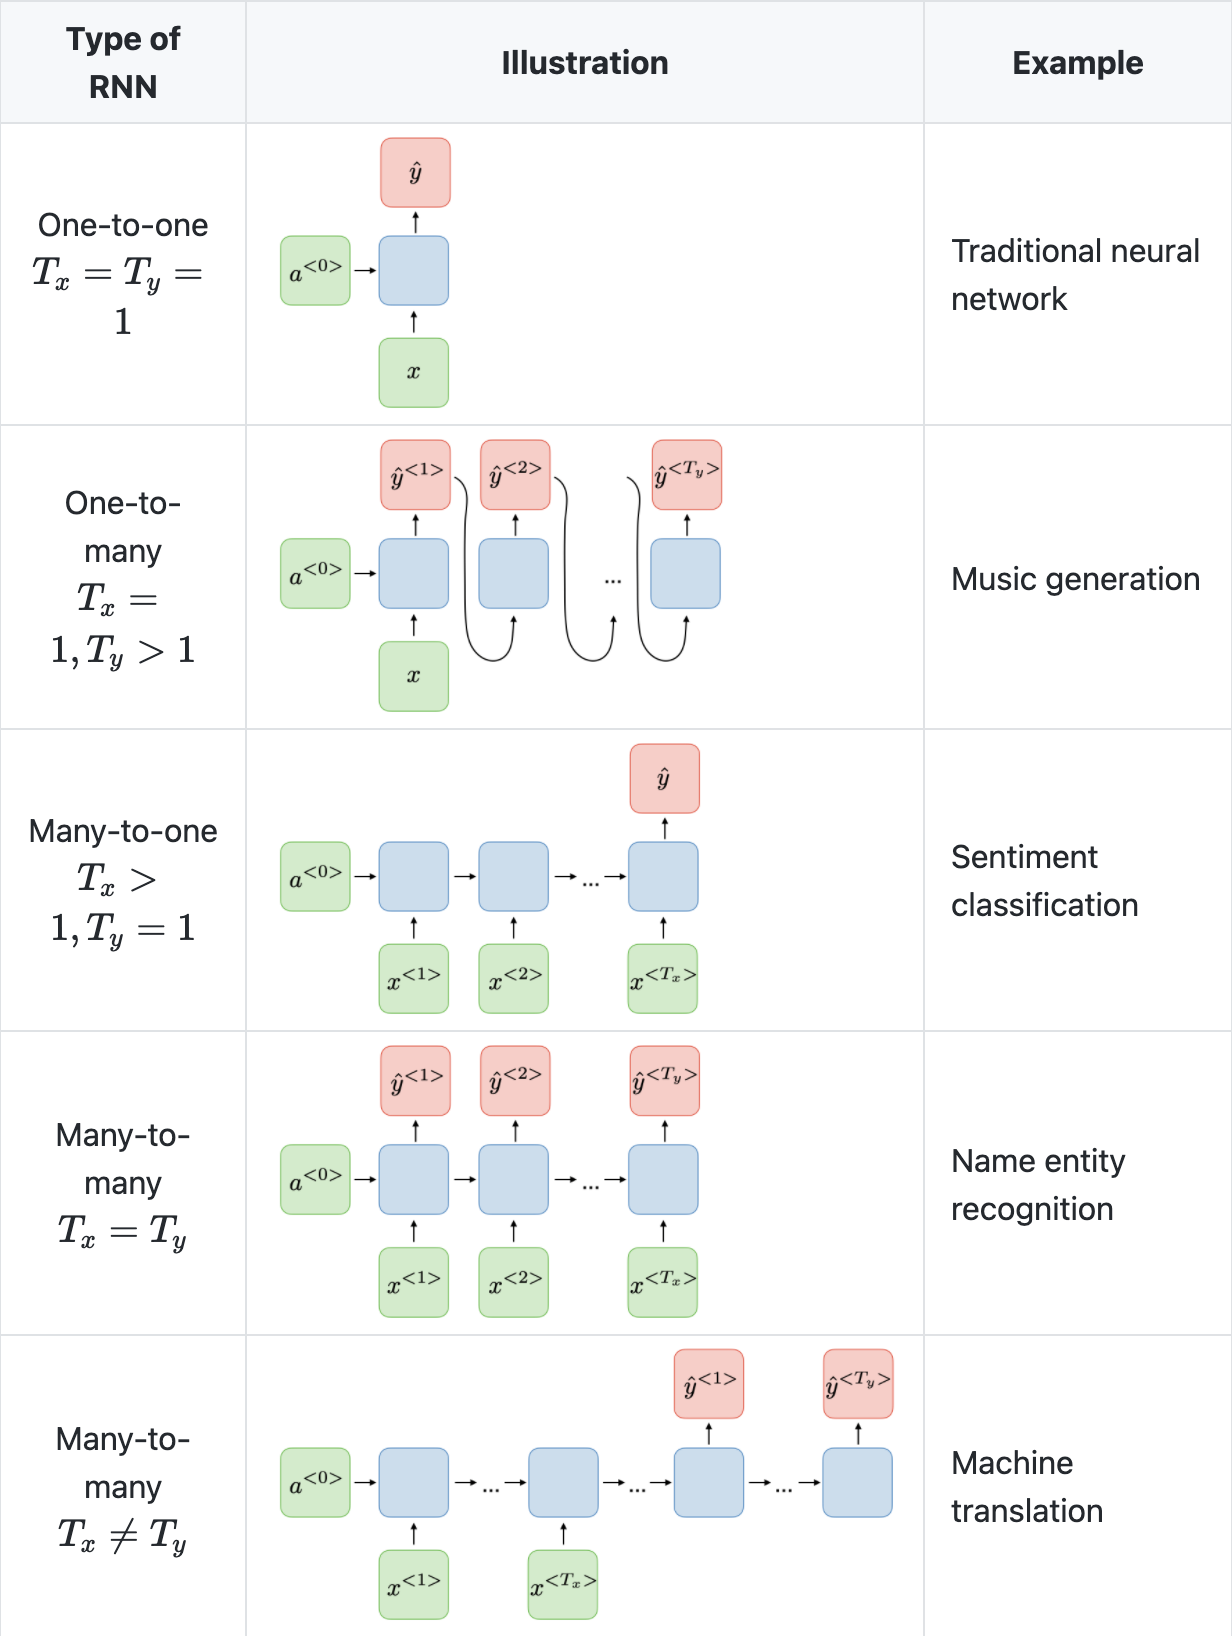
\includegraphics[width=0.8\textwidth]{stanford.edu__shervine_teaching_cs-230_cheatsheet-recurrent-neural-networks.png}
\end{figure}

Loss: accumulate all time stamp's loss

Backpropagation is done at each point in time. At timestep T, the derivative of the loss $\mathcal{L}$ with respect to weight matrix W.

The vanishing and exploding gradient phenomena are often encountered in the context of RNNs. The reason why they happen is that it is difficult to capture long term dependencies because of multiplicative gradient that can be exponentially decreasing/increasing with respect to the number of layers. Always, we capping the maximum of gradient to remedy this problem.

We can use several technical methods to optimize the RNN. 
\begin{itemize}
    \item Stack (cascade) RNN to make the model more complexed.
    \item bi-direction RNN. Just two RNN and concat the their results
    \item pretrain the embedding layer
\end{itemize}

If we want to predict an character, we can use character-level sequences to do the prediction.

During prediction, we can use temprature to improve the probability of the higher-prob char.

encode-decode the init input of decoder is the start sign.

bidrect as encoder + decode the performance is better.
\subsubsection{LSTM}
\begin{itemize}
    \item Update gate $\Gamma$ How much past should matter now?	GRU, LSTM
    \item Relevance gate $Gamma$ Drop previous information?	GRU, LSTM
    \item Forget gate F Erase a cell or not?	LSTM
    \item Put gate How much to reveal of a cell?	LSTM
\end{itemize}
\begin{figure}[htbp]
\caption{GRU versus LSTM}
\centering
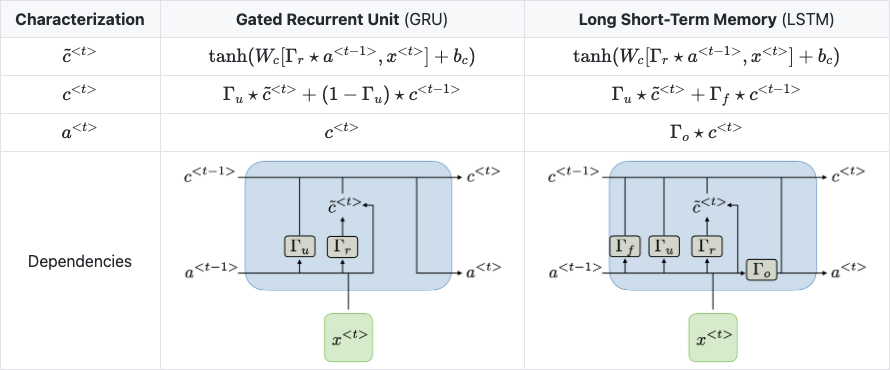
\includegraphics[width=0.8\textwidth]{stanford.edu__shervine_teaching_cs-230_cheatsheet-recurrent-neural-networks-2.png}
\end{figure}
\subsubsection{attention}
The first paper try to use attention in seq2seq is Neural Machine Translation by Jointly Learning to Align and Translate~\cite{bahdanau2014neural}. It seems that we aggregate a signle features and use the relationships between the all the hidden feature with the final features in the encoding.

the original paper: v inner product tanh(a single w * concat(final h = $s_0$, old state hi)) => real value. final h for each state s will generate a value alpha. We then softmwax the alpha.

Transformer one: ki = Wk * $h_i$ , q0 = Wq*s0;  ki*q0 = weight. Others is the same as above. So here, we adjust to a single w to two w. W key for the h and W query for the s.

alpha1 * h1 + .... alpha hn = c. Then we concat c in the decoder input.

And each time, we use the Wq*s1 .. Wq*s2.... n.  query for the decoder. each time we need to preserve the h1*Wk and recalculate Wq*s* [Wk*h1 ... Wk*hm] and it will cost m weights calculation. Therefore, it's depended on the seq length.

\textbf{self-attention}

Through the RNN, we can continue using hidden state to calculate c1 c2 c3... for example, if we want to calcualte c3, c3 = Wk*h1*Wq*h3*h1 + Wk*h2*Wq*h3*h2 + Wk*h3*Wq*h3*h3. Less likely to forget.

\textbf{Transformer}

Essentially, we use query for the hidden state to compute the relationship between the key value. And instead of using hi we can use Wv*hi.

How to remove RNN in the attention layer.

Instead of using the hidden state - the rnn output we can use the input directly. Thus (K*Q*v1)*V is the final answer of K*Q => weight, weight * V => final answer.

for each query, the input of the encoder is the original input and the last output of the attention layer.  So we can input the last round's correct answer as the input and the output of the attention layer shall be the next words. 

For the self attention, we map the each input to a query value qi.  The parameters are three weights matrix Wk Wq Wv.

self attention = single - head self attention head.  l head we can have 3l head matrices. We can stack the multiple results of multiple attention layer. 

Then we cascade the multi-head self layer we can generate the final results. (self-attention + dense) = block + resnet skip. IF we have different length for the input and output, we must use a encoder and decoder.

multiple blocks encoder => genereate u1 ... um, then we use attention again. We can use multi head attention to generate mutiple output of x1 .. xt, c1 ... ct then we can calcualte the K*Q*xt*V

But the output actual use a multi head self attention layer. We can generate c1 .. ct. Then we use multi head attention layer for u1 ... um and c1 ... ct to generate z1 ... zt and use dense network to generate the final results.

Therefore, we use encoder as 6 self attention + dense blocks. Then using the results as the input for the attention layer combined with self attention of the correct output. And then the multi head attention layer can generate a final state then using the dense net work to generate the final results.

(encode (self + dense) + self attention) * multi-head attention * dense = final resulst. We can stack the self attention and multihead attention layer again.

The attention is all you need~\cite{vaswani2017attention}

\textbf{Bert}

1. mask words to pretrain the encoding
2. predict next sentences through BERT

\subsection{Pytorch Tutorial}
\begin{itemize}
    \item the model will call the forward process directly if we initialize a model with a forward process in it.
\end{itemize}

\subsection{Meta-Learning}
\subsection{NAS}
\subsubsection{one shot learning}
\subsubsection{few-shot Neural Architecture Search}
\emph{Insights:}
Insight 1: When shall we stop? Use a GAP.
Insight 2: Why we always split the NN in the begining instead of during the experiments (DFS or BFS?) How to search efficently.
What can we split first? Choose the best then the edge.

\subsubsection{AutoFormer: Searching Transformers for Visual Recognition}
Previous works on designing vision transformers are based upon manual crafting, which heavily relies on human expertise and typically requires a deal of trial-and- error ~\cite{yuan2021tokens, touvron2021training, dosovitskiy2020image},.

we propose a supernet training strategy called weight entanglement dedicated to transformer architecture. The central idea is to enable different transformer blocks to share weights for their common parts in each layer. An update of weights in one block will affect all other ones as a whole,

This strategy is different from most one-shot NAS methods \cite{guo2020single, chu2021fairnas, wu2019fbnet}

it allows a large number of subnets in the super-net to be very well-trained, such that the performance of these subnets with weights inherited from the supernet are comparable to those retrained from scratch.

To tackle the challenges, we construct a large search space covering the main changeable dimensions of transformer, including embedding dimension, number of heads, query/key/value dimension, MLP ratio, and network depth.

To address the efficiency issue, inspired by BigNAS \cite{yu2020bignas} and slimmable networks \cite{yu2020bignas, yu2018slimmable}

It allows a large number of subnets in the supernet to be very well-trained, such that the performance of these subnets with weights inherited from the supernet are comparable to those retrained from scratch.

We perform a evolutionary search with a model size constraint over the well-trained supernets to find promising transformers.

Given a 2D image, we first uniformly split it into a se- quence of 2D patches. A transformer encoder consists of alternating blocks of multihead self-attention (MSA) and multi-layer perceptron (MLP) blocks. LayerNorm (LN) [2] is applied before every block, and residual connections after every block.

weight entanglement:

where W is the weight of the supernet, W is shared across all the architecture candidates
Since it is impossible to enumerate all the architectures $\alpha in A$ for evaluation, prior works resort to random search [34, 4], evolution algorithms [43, 16] or reinforcement learning [40, 48] to find the most promising one.

directly apply one-shot NAS for transformer search following classical weight sharing strategy [16], using differ-ent weights for different blocks in each layer, because of the slow convergence and unsatisfactory performance. The reasons: 1. The reason might be that the independent training of transformer blocks results in the weights being updated by limited times. 2. The perfor- mances of subnets inheriting weights from the one-shot su- pernet, trained under classical weight sharing strategy, are far below their true performances of training from scratch. 

The underlying reason is that homogeneous blocks are structurally compatible, such that the weights can share with each other. During implementation, for each layer, we need to store only the weights of the largest block among the n homogeneous candidates. The remaining smaller build- ing blocks can directly extract weights from the largest one.

During training, all possible subnets are uniformly sampled, and the corresponding weights are updated.

Such partition allows the search algorithm to concentrate on finding models within a specific parameter range, which can be specialized by users according to their available resources and application requirements.

For mutation, a candidate mutates its depth with probability Pd first. Then it mutates each block with a probability of Pm to produce a new architecture.

\emph{Insights:} 
1. For the weight entanglement, can we select several blocks to combine them as a more effective sub-supernets?  2. Use scrath result in better performance?
\subsection{Hyper Dimension Computing}
\subsubsection{Scalable Edge-Based Hyperdimensional Learning System with Brain-Like Neural Adaptation}
abstract:
Existing sophisticated algorithms such as deep learning are often overcomplex to run on less-powerful and unreliable embedded IoT devices. 

\section{Learn: Virtualization}
\section{Conference \& Talk}
\section{Research Project}
\subsection{Image Generation}
I take all notes in the another document
\subsection{SparseKernelSystemIntegration}
\subsubsection{TODO LIST:}
\begin{itemize}
    \item 1. Run fast transformer to see if I can actually print some useful information
    \item 2. find calling chain do we call these four GEMM functions 
    \item 3. find the weights if the other part of code use
    \item 4. Understand how the code to preserve cuda pointers for the weights \& design how to process these pointer to sparse format
\end{itemize}
\subsubsection{Insights:}
\begin{itemize}
    \item 1.
\end{itemize}
\subsubsection{Fast Transformer Coding}

\subsection{Pre-Expedite: Use Hierarchical Structure Space for Improving the Performance of Accessing Small Files in Parallel File System}
\subsubsection{TODO LIST:}
\begin{itemize}
    \item 1. Review the paper
    \item 2. Re-organize the reference and read the paper
    \item 3. Revise the paper
\end{itemize}
\subsubsection{Insights:}
\subsubsection{DeltaFS: Exascale File Systems Scale Better Without Dedicated Servers}
\subsubsection{DeltaFS: A Scalable No-Ground-Truth Filesystem For Massively-Parallel Computing}

\subsection{MAEE - Multiple Applications Execution time Estimation}
\subsubsection{TODO LIST:}
\begin{itemize}
    \item 1. Read the original paper and split it into profiling paper part
    \item 2. Read the current benchmark papers and do some profiling experiments
    \item 3. Read analysis paper and analyze the profiling results
\end{itemize}
\subsubsection{Insights:}
\begin{itemize}
	\item make a open-source dataset for the applications 
	\item Design an accurate model for co-running them with the fact of time shifting. Esitimate the future running time.
	\item Label different kind of applications
	\item What is the realistic scenario for the scheduling problem?
    \item For the related work, we know that there are several works before. They focused on 1. dynamic or static 2. optimize different features (Cache, Memory access, etc) to let the features be more accurate. 3. dd new features 4. Modify the model
    \item current datasets: 1. SPEC 2006 2. NPB applications with high memory intensity (e.g., soplex, libquantum, mcf ) and high cache sensitivity (e.g., ft, dealII, bzip2). TPC-C [68] and the Yahoo Cloud Serving Benchmark (YCSB) HiBench [10], Spark-perf [12] and SparkBench [11]. Shuhai benchmark
    \item What is the boundary of ML applied in the scheduling?
\end{itemize}

What we want to do?:
\begin{itemize}
    \item 1. Select 1000 benchmarks and do the classification for these applications. We choose several dimension to classify: 1. HPC,ML,BIG DATA 2. compute-bound, network-bound, memroy-bound
    \item 2. When we co-execute these applications, the interface between them and relationship between the dimension supervised together.
    \item 3. Profiling results
\end{itemize}
\subsubsection{perf-tools}
\begin{itemize}
    \item nsys
	\item perf perf stat Run a command and gather performance counter statistics -I msecs -a, --all-cpus system-wide collection from all CPUs (default if no target is
specified) -x SEP, --field-separator SEP print counts using a CSV-style output to make it easy to import directly into spreadsheets. Columns are separated by the string specified in SEP. -e a symbolic event name (use perf list to list all events) a raw PMU event (eventsel+umask) in the form of rNNN where NNN is a hexadecimal event descriptor. -p, --pid stat events on existing process id (comma separated list) perf list cpu/t1=v1[,t2=v2,t3 ...]/modifier                  [Raw hardware event descrip (see 'man perf-list' on how to encode it)
	\item iostat
	\item vmstat
	\item ifstat
\end{itemize}

\subsubsection{The Application Slowdown Model: Quantifying and Controlling the Impact of Inter-Application Interference at Shared Caches and Main Memory}

abstract: Unfortunately, prior works on estimating slowdowns either lead to inaccurate estimates, do not take into account shared caches, or rely on a priori application knowledge. ASM that accurately estimates application slowdowns due to interference at both the shared cache and main memory.  1. minimizes interference for the application at the main memory, 2.quantifies the interference the application receives at the shared cache Usage: slowdown-aware cache partitioning, slowdown-aware memory bandwidth parti- tioning and an example scheme to provide soft slowdown guarantees. (rate means speed of accessing rate)

background, motivation: profiling before or not?  no free resources, foreground and background jobs are run together, input set dependent => it's hard to estimate its alone execution time online.   by observing its aggregate request service behavior rather than individual request service behavior to quantify interference.  the performance of each application is roughly proportional to the rate at which it accesses the shared cache.   an application’s slowdown depends on the sensitivity of its performance to cache capacity and memory bandwidth, making online slowdown estimation a hard problem.  

related work: Fairness via Source Throttling (FST) \cite{ebrahimi2010fairness}  and Per-thread cycle accounting (PTCA) \cite{du2013per} estimate slowdown due to both shared cache and main memory interference While several prior works (e.g., \cite{ebrahimi2010fairness,du2013per, mutlu2007stall,subramanian2013mise}) proposed online mechanisms to estimate application slowdowns either inaccurate and/or do not take into account shared caches. FST, PTCA determine the number of cycles by which each request of the application is delayed due to interference at the shared cache and main memory.   STFM \cite{mutlu2007stall} making it difficult to accurately estimate the interference cycles for each application. FST uses a pollution filter for each appli- cation that tracks the blocks of the application that were evicted by other applications. PTCA uses an auxiliary tag store. But they are inaccurate. First, both FST and PTCA quantify interference at an individual request granularity.  In fact, MISE \cite{subramanian2013mise} observes that the performance of a memory-bound application is proportional to the rate at which its memory accesses are served.

motivation: A shared cache only makes the problem worse as the request stream of an application to main memory could be completely different when it shares the cache with other applications versus when it runs alone.  interference behavior varies widely across requests and is difficult to estimate accurately by sampling and scaling. ASM build an accurate, low- overhead, online model

Design: by using an auxiliary tag store [53,56] to determine the number of shared cache misses that would have been hits if the application did not share the cache with other applications This aggregate contention miss count is used along with the average miss service time (from the previous step) to estimate the time it would have taken to serve the application’s requests had it been run alone.   $slowdown = \frac{performance_{alone} ~ CATCH_{alone}}{performance_{share} ~ CATCH_{share}}$ (CATCH means cache access rate) on the other hand, can be estimated more accurately by exploiting the observation made by several prior works that applications’ phase behavior is relatively stable over time scales on the order of a few million cycles.   online: it would not eliminate shared cache interference, since the caches cannot be warmed up at will in a short time duration.  Online cannot let the application run by itself to warm up the memory. Minimizing main memory interference, quantifying interference at the shared cache is another better choice to estimate $cache_{alone}$. 

Impelment: 

1.ASM divides execution into multiple quanta, each of length Q cycles $ CAR_{shared}$ Access / Q 

2. ASM divides each quantum into epochs of length E cycles (thousands of cycles)  $CAR_{alone}$   = $\frac{epoch-hits + epoch-misses}{(E*epoch-count) - (epoch-excess-cycles)}$   epoch-excess-cycles is the number of excess cycles spent serving the application’s contention misses—those that would have been hits had the application run alone.  epoch-excess-cycles = ($\sharp$ Contention Misses) × (avg-miss-time − avg-hit-time). $\sharp$ Contention Misses = epoch-ATS-hits − epoch-hits $avg-miss-time = \frac{epoch-miss-time}{epoch-misses}$ $avg-hit-time = \frac{epoch-hit-time}{epoch-hits}$ how many seconds one hit, one misses, we minus them we can get the second we shall not misses, the time seconds*misses => cycles. 

3. Mem Queueing delay to show cache alone, we give the application highest priority. But it's not enough. if we do not schedule this highest priority application, but other app submit, they will be scheduled. Later, the highest priority will be delayed. the author take this as the ATS misses. and $avg-queueing-dealy = \frac{\sharp queueing cycles}{epoch-misses}$ $CAR_{alone} = \frac{as-above}{(as-above) - (epoch-ATS-misses*avg-queueing-delay)}$ ATS means we can hit alone, hit is real hit. The diff is the contention miss.

4. Overhead => dynamic cost because it need to store the queueing cycles and several variables

EXP:

similar to Ramulator \cite{kim2015ramulator}. We validated the simu- lator against DRAMSim2 \cite{rosenfeld2011dramsim2} and Micron’s behavioral Verilog model [41]. https://github.com/CMU-SAFARI. SPEC CPU2006 [4] and NAS Parallel Benchmark

We compute IPCalone for the same amount of work com- pleted in the alone run as that completed in the shared run for each quantum.

1 error,  2 latency. 3 we seek to isolate the benefits of using epoch-based aggregation to account solely for memory interference from the benefits of using epoch-based aggregation for both main memory and shared cache interference. 4 ensitivity to System Parameters a Core count. why accuracy decrease? However, the effect of this queueing is greater at higher core counts and is harder to account for entirely. b capacity of cache size c quantum length and epoch length

leveraging ASM:

1. Cache partitioning 1. $slowdown_n = \frac{CAR_{alone}}{CAR_n}$  the core idea is to esitmate $CAR_n$ only we update cache policy to n-way cache we can know. But we can estimate by ASM. Also the challenge is to meansure the number of cycles to serve an application. The author use miss - hit as the excess cycles 2. we use the look-ahead algorithm used in Utility-based Cache Partitioning (UCP) [56] to partition the cache ways such that the overall slowdown is minimized. $slowdown-utility^{n+k}_n = \frac{slowdown_n - slowdown_{n+k}}{k}$  For more details on the partitioning algorithm, we refer the reader to \cite{qureshi2006utility}. The author use harmonic speedup to evaluate the ASM.


\emph{Insights}: 

1. I guess ASM want to predict in the runtime, thus, it need to reduce interference and use the cache access manners to predict the interference 

2. different dimensional of current methods: a. profiling or not profiling b. online or offline c. two or multiple d. offset of applications e. complexity of model 

3. ASM only roughly connect performance of model to the proportional to the rate at which it access the shared cache 

4. 考虑到GPU程序,资源冲突上有没有什么区别? GPU版本 + CPU版本 

5. Can we find some patterns co-running applications. 

6. Memory Bound (Data cannot serve) + Comput Bound (Data can serve) => Memory Bound*2? 

7. They ignore the compute intensive?

8. 长时间的特征变化肯定是不一样的,需要用cach alone 时序数据而不是时刻数据去做预测. 文章是用每秒平均的cache关系去做一些分析

\subsubsection{Sequence-to-sequence models for workload interference prediction on batch processing datacenters:}

Since the average utilization is estimated to be below 50\%~\cite{barroso2007case, reiss2012heterogeneity} The principal problem when co-locating resource-sharing ap- plications is to ensure that competition will not ruin their QoS,

Since interference creates a new characteristic footprint for each set of concurrent applications. Applications can be profiled in isolation in order to characterize the requirements claimed during their execution. Thus, there is the need to predict application resource demands and interference without the burden of running all possible combinations of applications.

Therefore, they produce a single value global prediction estimate, instead of a sequence of predictions over time. Most classic machine learning approaches for this problem, such as ~\cite{mishra2017esp, delimitrou2013paragon}, do not consider the temporal dimension of executions.

Our model employs two Gated Recurrent Units (GRU) [9] as building blocks; one GRU processes the trace signal of the incoming applications and passes the processed information to the other GRU, which outputs the expected resources of the co- located applications over time.

Intel HiBench [10], the IBM SparkBench [11] and the Databricks Spark-Perf benchmarks [12]

\begin{itemize}
	\item  A novel use of Recurrent Neural Networks that estimates the monitored metrics of two co-scheduled applications $a \wedge b$ from the information of a and b gathered running the applications in isolation.
	\item A novel feature, percentage completion time, for estimat- ing the completion time of co-scheduled applications. This feature improves predictions made by using the standard stopping criteria based on the end of sequence feature.
	\item A comprehensive evaluation of the method against other relevant machine learning approaches. We show the advan- tages of our method, which are especially noticeable in two cases: when co-located executions have different lengths, and when co-scheduling heavily impacts the execution time of the applications due to high interference.
\end{itemize}

The way in which st is computed is what mostly differentiates RNN models, such as Gated Recurrent Units [9] (GRU) and Long Short- Term Memory [13] (LSTM).

The decoder reads the encoded vector and produces a new sequence, but instead of initializing the hidden state of the decoder with zeros, it is initialized to the last hidden state of the encoder RNN

the context vector is computed as a matrix vector product, which can be interpreted as a weighted sum of the columns of E. The encoder generate this matrix E directly and multiply matrix E with the input, last state and finally use E and vt to generate a fixed size sequences. The input of decoder are context vector generated by the input vector, last hiden state input, 

EOS. This feature vector takes value 0 at every time step except the last one, where it takes value 1. This vector simply tells the decoder when both applications finish.

In that scenario, EOS is just a special word that stops the decoding process, which means that if the decoder emits the ‘‘EOS’’ symbol the decoding process is stopped. In our setting the EOS is a new feature that takes a real value at every time step.

We denote by PCFa and PCFb the percentage completion features for input sequences a and b, respectively. Both features contain at time t how much of the workload has been completed until t, expressed as a percentage. For a given sequence s of length N, we define PCFs = (1 ·100, 2 ·100,..., N ·100). Notice that, by construction, PCF features contain monotonically increasing values that must finish with value 100. Nevertheless the rate of increment at every time step will depend on the overall number of time steps of the sequence.

vmstat, iostat, ifstat and perf. The dataset used in the experiments contains traces generated by a variety of micro-benchmarks (workloads). The workloads used have been extracted from different suites: HiBench [10], Spark-perf [12] and SparkBench [11]. 

The author have three other model - basline model - ioslated prediction. The degradation of quality for long sequence prediction is a known issue found

Since we do not know in advance how long co-scheduled applications can take to finish, we have decided to treat the length of the generated trace as a hyperparameter to be adjusted. The different criteria tested are as follows:

applications are predicted to finish the larger the expected error. The box plot shows results for the criterion argmax PC sum

then errors are large because the stopping criteria is fired before the co-scheduled applications might finish. Errors decrease as k increases up to a point where the errors start to increase.

dynamic provisioning and job placement. predict whether there will be a change in the workload trace that needs some hardware decision. 

Works like \cite{islam2012empirical, kumar2018workload} use neural networks that take as input resource usage in a given time window with the goal of predicting the future resource requirements for the workloads. In authors use differential evolution as a means to train the models, whereas in they use standard gradient based algorithms.

In \cite{zhang2016workload}, RNNs are used to predict cloud resource requests of Google cloud CPU and RAM requests, results are compared against ARIMA forecasting, achieving lower error with the RNN. they do not take into account the degradation of the applications under co-scheduled scenarios or the challenges that appear when a full time series is meant to be predicted from more than a input trace signal.

\cite{marco2017improving} it then passes through a k-Nearest Neighbor in order to choose the most representative expert. Finally, the application is run with different data sizes in order to tune the function parameters to determine the best fit for this application. 

SVD and PQ-reconstruction [29]. In Paragon, the profiling across pairs is limited to the first minute due to time constraints, without covering applications with different execution phases and behaviors over time

properly ensure resource availability for specific jobs. Such a solution tends to overresource applications for solving the interference problem, thus becoming subject to machine under-utilization. Another interesting work dealing with protection against in- terference is Stay-Away by \cite{rameshan2014stay}

In \cite{wyatt2018prionn} the authors present a convolutional neural network named PRIONN. The model predicts run-time and IO (bytes read and total bytes written) of applications based on the source code in the input script. 

In \cite{berral2015aloja} Aloja-ML is presented as a framework for character- ization and knowledge discovery in Hadoop deployments. The authors present different methods for execution time prediction based on hardware resources, workload type and input data size.

\emph{Insights}: 

1. not consider multiple applications are running in the nodes. $a^b$ represents an execution of the co-located pair. $a^{\rightarrow} \wedge b$ For the percentage completion time, 

2. Can we use a unsupervised learning algorithm for this problem?  to do a classification for the program?  Like the roofline model? I can try this.

3. No one use a SPEC, NPB HPC benchmark.

4. The author do not consider other time-series model as comparison

5. Can we abandon the EOS or PC and focus on time estimation?

6. Can we design one NN for one index?

7. Can we focus on more combination of system profiling?

8. profiling slowdown

9. what is exactly usage of EOS or PCF?


\subsection{Hybrid - Share: Resource Management System}
\subsubsection{TODO List:}
\begin{itemize}
    \item 1. Read more scheduling papers
    \item 2. think about combine my profiling algorithm with scheduling algorithm
    \item 3. Deploy scheduling papers' open-source repo \& Write my own scheduling or simulator scheduling papers
\end{itemize}
\subsubsection{Insights:}
\begin{itemize}
    \item I found an interesting insights in my past paper. The layout affects the interference of two applications. Balance and Continous. Maybe I can keep doing the research of this part.
    \item neglect the impact of for one tasks, may have some master-slaver mode. The resources consumption is not homogeneous.
    \item biparitate match is not the best. It cannot solve the problem of several jobs running together. It can olny deploy two jobs togther. It's worth mentioning that HybridShare neglect to place the multiple jobs in the job queues to the same nodes.
    \item Can we use the algorithm into the cloud computing
\end{itemize}
\subsubsection{Topology-Aware Scheduling System}
\subsubsection{Scheduling Scenario - Theory and Practice in Parallel Job Scheduling}
\subsubsection{Differentiate Quality of Experience Scheduling for Deep Learning Inferences with Docker Containers in the Cloud}
However, cloud providers fail to offer a QoE-based option to their clients. Clients have to balance the budget and quality of expesystem
riences (e.g., response time). DQoES accepts clients’ specifications on targeted QoEs, and dynamically adjusts resources to approach their targets. 

Pros: 1. the author finds a good cut-off to introduce their idea, to focus on differentiating QoEs for deep learning backend inferences. 2. The paper design two algorithms, one for deciding the resources limit for the container to approach the QoS target and another for reducing adjustment overhead at each time point.

Cons: A. Typos and Ambiguous: 1. page2 line44 shall be back-end instead of backed 2. It is ambiguous of the number of workers and the meaning of the purple rectangle in the figure 1 3. what does page 3 line 39 'each deep learning model that runs this worker.' mean? 4. why workers monitor track models instead of tracking workers' performance? 5. It's messy to organize the all kinds of monitors in figure 1 6. Table I shall use $T_{R_i}$ instead of $T_R$ 7. The table I does not explain the meaning of set C 8. what does $R_g$ resource usage mean in the Table I? CPU, mem or ? B. Ideas: 9.  $1− \frac{q_i}{Q_G}×R_Gx\beta$ does $R_G*\beta$ will be bigger than 1? How to limit $1− \frac{q_i}{Q_G}×R_Gx\beta$ does $R_G*\beta < 1$  10. why the algorithm only focus on the CPU usage to represent the resource demand for the deep learning model? 101 The paper does not explain why the limit of resources for a model is related to the global QoS target - $\frac{q_i}{Q_G}$ in Line 18 in algorithm 1 12. Many parameters in an algorithm cannot understand until reading your experiments. 13. The paper lack overhead, throughput, scheduling integration, and resources usage assessment. And what is GPU setting in the experiment and the size of nodes are too small to simulate a cluster environment 134 The paper does not handle the resource contention slowdown between these containers. Does the author consider the resources are not infinite and adjust sharing resources may result in slowdown of model inference? 15. I don't see any effect of IV variable in algorithm 2 16. Under the limited resources, the author said could to approach the targets by evenly distributing all the resources. Can we restrict part of the service to reach other models' target QOS?  17. the paper shall compare more with the Qos aware scheduling algorithm (e.g., ASPLOS 2021 Sinan: ML-Based and QoS-Aware Resource Management for Cloud Microservices) 18. Docker Swarm contains a lot of load-balance policy,  it's unfair to say 'Docker Swarm places containers based on the number of containers on each worker and assumes each container allocates an equal share of resources'.  

Overall, authors shall take more effort to explain the intuition of two algorithms and reorganize the order of content of the paper to explain each details of the concept in the algorithms. Also, there is a space to improve the experiment.

background: 1 balance the budget from its own end and deliver the quality of experiences .2. different applications lead to various QoEs requirements. 3. they are provided with various resource levels. These levels fail to link to QoEs directly => fill the gap 该文章想把QOS level和resource level 做一个绑定 这是一个好的想法? it is a challenge to differentiate the deep learning inferences, which require micromanagement on the resources of each task at runtime. 4. alpha 算法没有给出解释 后面实验需要给出

related work: ProCon [23] optimizes the cluster by selecting a best-fit host for incoming tasks Clockwork [27] exploits predictable execution times of deep neural network inference. Optimus [26] employs an online fitting technique to predict model convergence and sets up performance models to estimate training speed.  FIRM [28] considers the resource sharing. It reduces the SLO violations by lever- aging online telemetry data and utilizing a support vector machine based model to identify the key components that are likely to become resource bottlenecks. AI4DL [29], [36] studies the training processing of deep learning applications within IBM’s DLaaS containers. It demonstrates that CPU and memory usage can be reduced significantly by leveraging typ- ical resource usage patterns.

Design: the target of system is to minimize the the models in the category perform better/poor than the preset QoE value, and sum o-p (target - performance).  Why the qi = oi - pi?  It seems the author use a $1− \frac{q_i}{Q_G}×R_G ×β$ * last time resources to tune the resource limit. BUT WHY one model's resource limit is related to other QOS target of containers? And the overhead to adjust the constraint? 

Exp: why only the applications focus on the cpu usage? We can also draw a graph to track the job trace  how to move the application between the node to improve the QOS? QOS aware -> We will design container placement and migration strategies with respect to the states of worker nodes.  Use a model to predict the QOS slowdown.

\emph{Insights}: 
1.Use a model to predict the QOS slowdown. (given resources to predict QOS) \\
2.把QOS level和resource level 做一个绑定 这是一个好的想法 Given resources to predict the QOS
3. Draw a graph to trace a job to take this a feature of the job
\subsubsection{Job placement using reinforcement learning in GPU virtualization environment}

abstract: This study defines the resource utilization history of applications and proposes a reinforcement learning-based job placement technique, which uses it as an input. For resource utilization history learning, a deep reinforcement learning model (DQN) is used. 

background: Many large cloud providers, such as Amazon EC2 [1], Nimbix [2], Microsoft Azure [3], and Alibaba [4] provide GPU services. When a user requests a GPU, these service providers (e.g., Kubernetes [5], Mesos [6]) grant exclusive access rights to the user instead of on- demand access. NVIDIA has provided a Multi-Process Service (MPS) [12] that executes multiple applications in one process by GPU sharing. However, this technology can be helpful for performance improvement if, and only if the kernel pattern of the application is known. HPC+ML, 

related work: There are studies on the scheduling of co-execution tasks of applications in GPU resources: the co-placement method of applications is based on monitoring \cite{chang2017kubernetes,gu2018gaiagpu}, and a weight-based placement method using the GPU use profiling information of applications \cite{hong2017fairgv}.  

motivation:  VGG16, RESNET-50, LAMMPS, QMCPACK. the HPC applications have various resource utilization patterns depend- ing on the execution stage. For the comparison, we used three deep-learning applications (CNN, vgg16, googlenet) of TensorFlow benchmark showing similar resource utilization characteristics and two HPC applications (LAMMPS and GROMACS) of NGC (Nvidia GPU Cloud). Scheduling that predicts the performance by using a conventional heuristic method through the usages of each resource is an NP-hard problem. 

design: 1. describe multiple co-run applications 2. history of the application to be used for learning is defined 3. learning-based job placement method is proposed, which uses the defined resource utilization history as input.   1. Resource utilization history items of GPU application: 

\begin{figure}[htbp]
\caption{scheduling architecture}
\centering
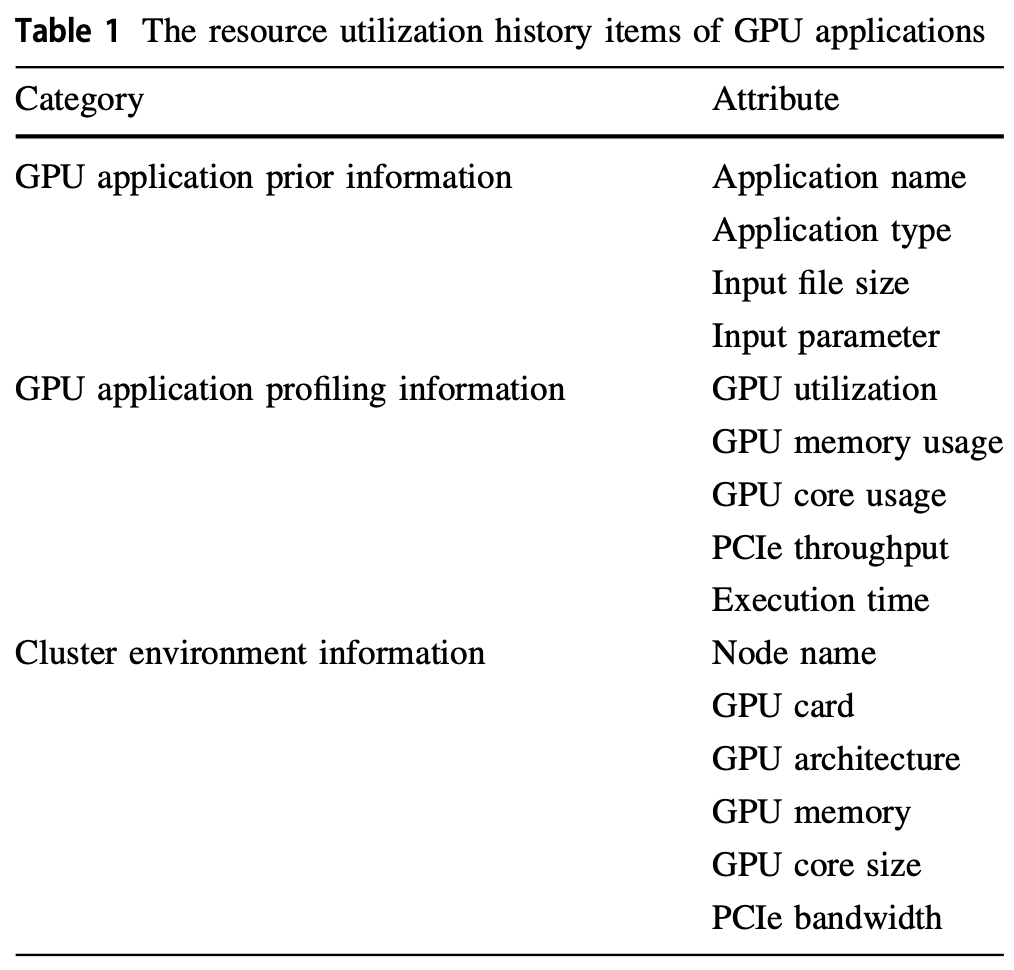
\includegraphics[width=0.8\textwidth]{GPUAPP.png}
\end{figure}
\subsubsection{Scalable system scheduling for HPC and big data}
\subsubsection{异构计算系统调度理论与方法}
背景:\\
1. 使用的计算资源具有多种类型的计算能力 SIMD MIMD 向量 \\
2. 不同计算类型的计算资源能够相互协调运行 \\
3. 不同子任务的并行性需求类型 \\
4. 并行性 + 异构性 \\
目标: 最短时间\\
网格GLOBUS: 构造层 - 连接层 - 资源层 - 汇聚层\\
CPU + 协处理器 GPU/MIC \\
云计算服务层次;1.应用层, 2.平台层(软件框架), 3. 基础设施层(系统资源访问, 资源管理系统), 4. 虚拟化层(容器)

任务调度:\\对MPI OpenMP等分布式并行应用程序进行任务分割; 调度任务可以分为动态,静态任务,局部,全局;t-level, b-level (静态的BL => SBL)  => ASAP,ALAP; 计算节点有限, 计算节点无限, 计算节点任意连接, 复制关键任务, DL动态级调度 - DL = SBL - EST(最早执行时间), MH算法 - SBL,HEFT 算法平均成本, wi + max(rank(successor)); In operations research, the makespan of a project is the length of time that elapses from the start of work to the end

基于动态通信竞争的调度算法:\\平均执行成本,优先权计算,动态通信竞争,最早最晚执行时间,通信边调度,LST,LFT, 通信竞争表调度算法 - Sinnen 通信计算比率 CCR => 低中高通量 并行调度 

任务复制调度策略: \\ \cite{zhao2003experimental} 根据异构处理机上的执行成本来进行任务调度对算法性能有深远影响。 处理机平均计算能力。异构通信链路因子。 list scheduling algorithm => In classical list scheduling algorithms an application is viewed as a directed acyclic graph (DAG), where nodes (or tasks) represent computation and edges represent communication. By assigning a weight to each node (typically, the corresponding computation cost) and edge (typically, the corresponding communication cost), those algorithms prioritize the nodes to be scheduled on the basis of a value computed by a rank function; this is typically a function of the weights assigned to the nodes and edges of the graph.  标准调度长度,  是否可以运用在某个大的应用内部 DRT 数据准备时间

可靠性感知的任务调度:\\ 故障率与系统规模的正相关, 位置局部性,与负载具有正相关,故障的传播性(积累)。软件容错模型: TMR,priamry backup model, spare processor model, imprecise computational model, m,k, firm deadline. Weibull 分布 异构计算系统失效率减少 增加或常量等特性。可靠性容错调度: 仅仅通过调度增加系统的可靠性,近几年可靠性成本融入经典调度DLS算法中。 可靠性调度模型: 一个典型调度系统包括 资源模型,工作流模型,调度体系结构和评价指标。schedule queue, dispatch queue. 可靠性分析: $LST(e_{i,j},l_1) = max(EFT(v_i), available(e_{i,j}, l_1))$. Weibull: 可靠性函数: R(t) = $e^{{-\frac{t}{\lambda}}^k}$ 失效率函数: $\frac{k}{\lambda^k}*t^{k - 1}$ 每一个处理器有一个 $\lambda$ ,$k$来控制 \cite{murthy2004weibull} 可以估计出 $\lambda$,$k$.  任务调度算法: 基于均值优先排序性质计算任务优先级, 优先级递归计算. 唐的算法加权可靠性成本和最早完成时间成本之和。基于simgrid唐完成了实验

网格分层调度理论:\\局部硬件资源。由于任意处理机网络构成的虚拟节点可能存在多条这种通信路径,因而查找最优可靠的通信路径是提高系统可靠性的有效途径。最早通信完成时间可能会受到动态通信链路的影响,静态Dijkstra选择最早的貌似不可取?  局部调度算法: 每个任务在每个处理机都给予一个系统开销然后挨个寻找最大的匹配?用完全图匹配是不是更好?有没有图匹配相关的调度算法?可靠性驱动的分层任务调度。其实通过模拟器方法,迭代修改算法也是发表论文的一个比较好的方法。模拟的时候,程序的相关信息都是全知道的,这个其实貌似在现实世界中感觉不太可能。。。所以其实在我的研究和传统调度算法研究中间是有gap的?

考虑任务执行行为的安全性调度方法:\\异构计算系统的安全可信性: 分布式信誉管理机制,高效的多QoS静态异构分布式的系统调度算法用于满足多用户并法安全性在内的多QoS需求。具体做法:  安全需求等级提前确定好。 安全需求主要的问题: 1. 缺乏委托机制 2.鉴权 3. 本地信任策略具有局部性 4. 安全表达能力与安全扩展性 信任=直接信任+声誉 一般假设任务执行行为安全性在固定时间间隔内服从泊松分布。发现一个问题,每个计算公式的加权和相处计算的直觉分别是什么?为什么要用这个公式?找个一个安全性概率小于常数$\theta$,安全性概率用来表明任意一台机器可能出错的概率。然后再找具有最早完成时间的任务集合。

任务计算量服从随机分布调度理论:\\ 通过每个任务完成时间的期望和方差,依据线性规划进行调度问题 的最优解分析。对具有指数分布的随机任务调度问题,应用LEPT。调度长度的标准方差。随机调度问题调度长度的期望值的下限是将任务计算量以期望值代替所得到的确定性任务调度问题的调度长度。以往的异构没有考虑的资源需求的多样性。选择一个任务时间优于另一个任务时间这种优于的概率高的。利用概率累计函数。

能耗感知随机任务调度策略:\\DFVS技术动态调节操作频率。Clark方程估计正态分布的最大值的期望值和方差。当我们有了每个处理器上随机调度时间最大值的期望,现在要这个期望<d代表所有任务都在d内完成,这个P(<d)变成了累计分布函数CDF。算法加权能耗概率和任务完成时间概率。应用:mpegplay,madplay,tmndec,toast

\begin{figure}[htbp]
\caption{scheduling architecture}
\centering
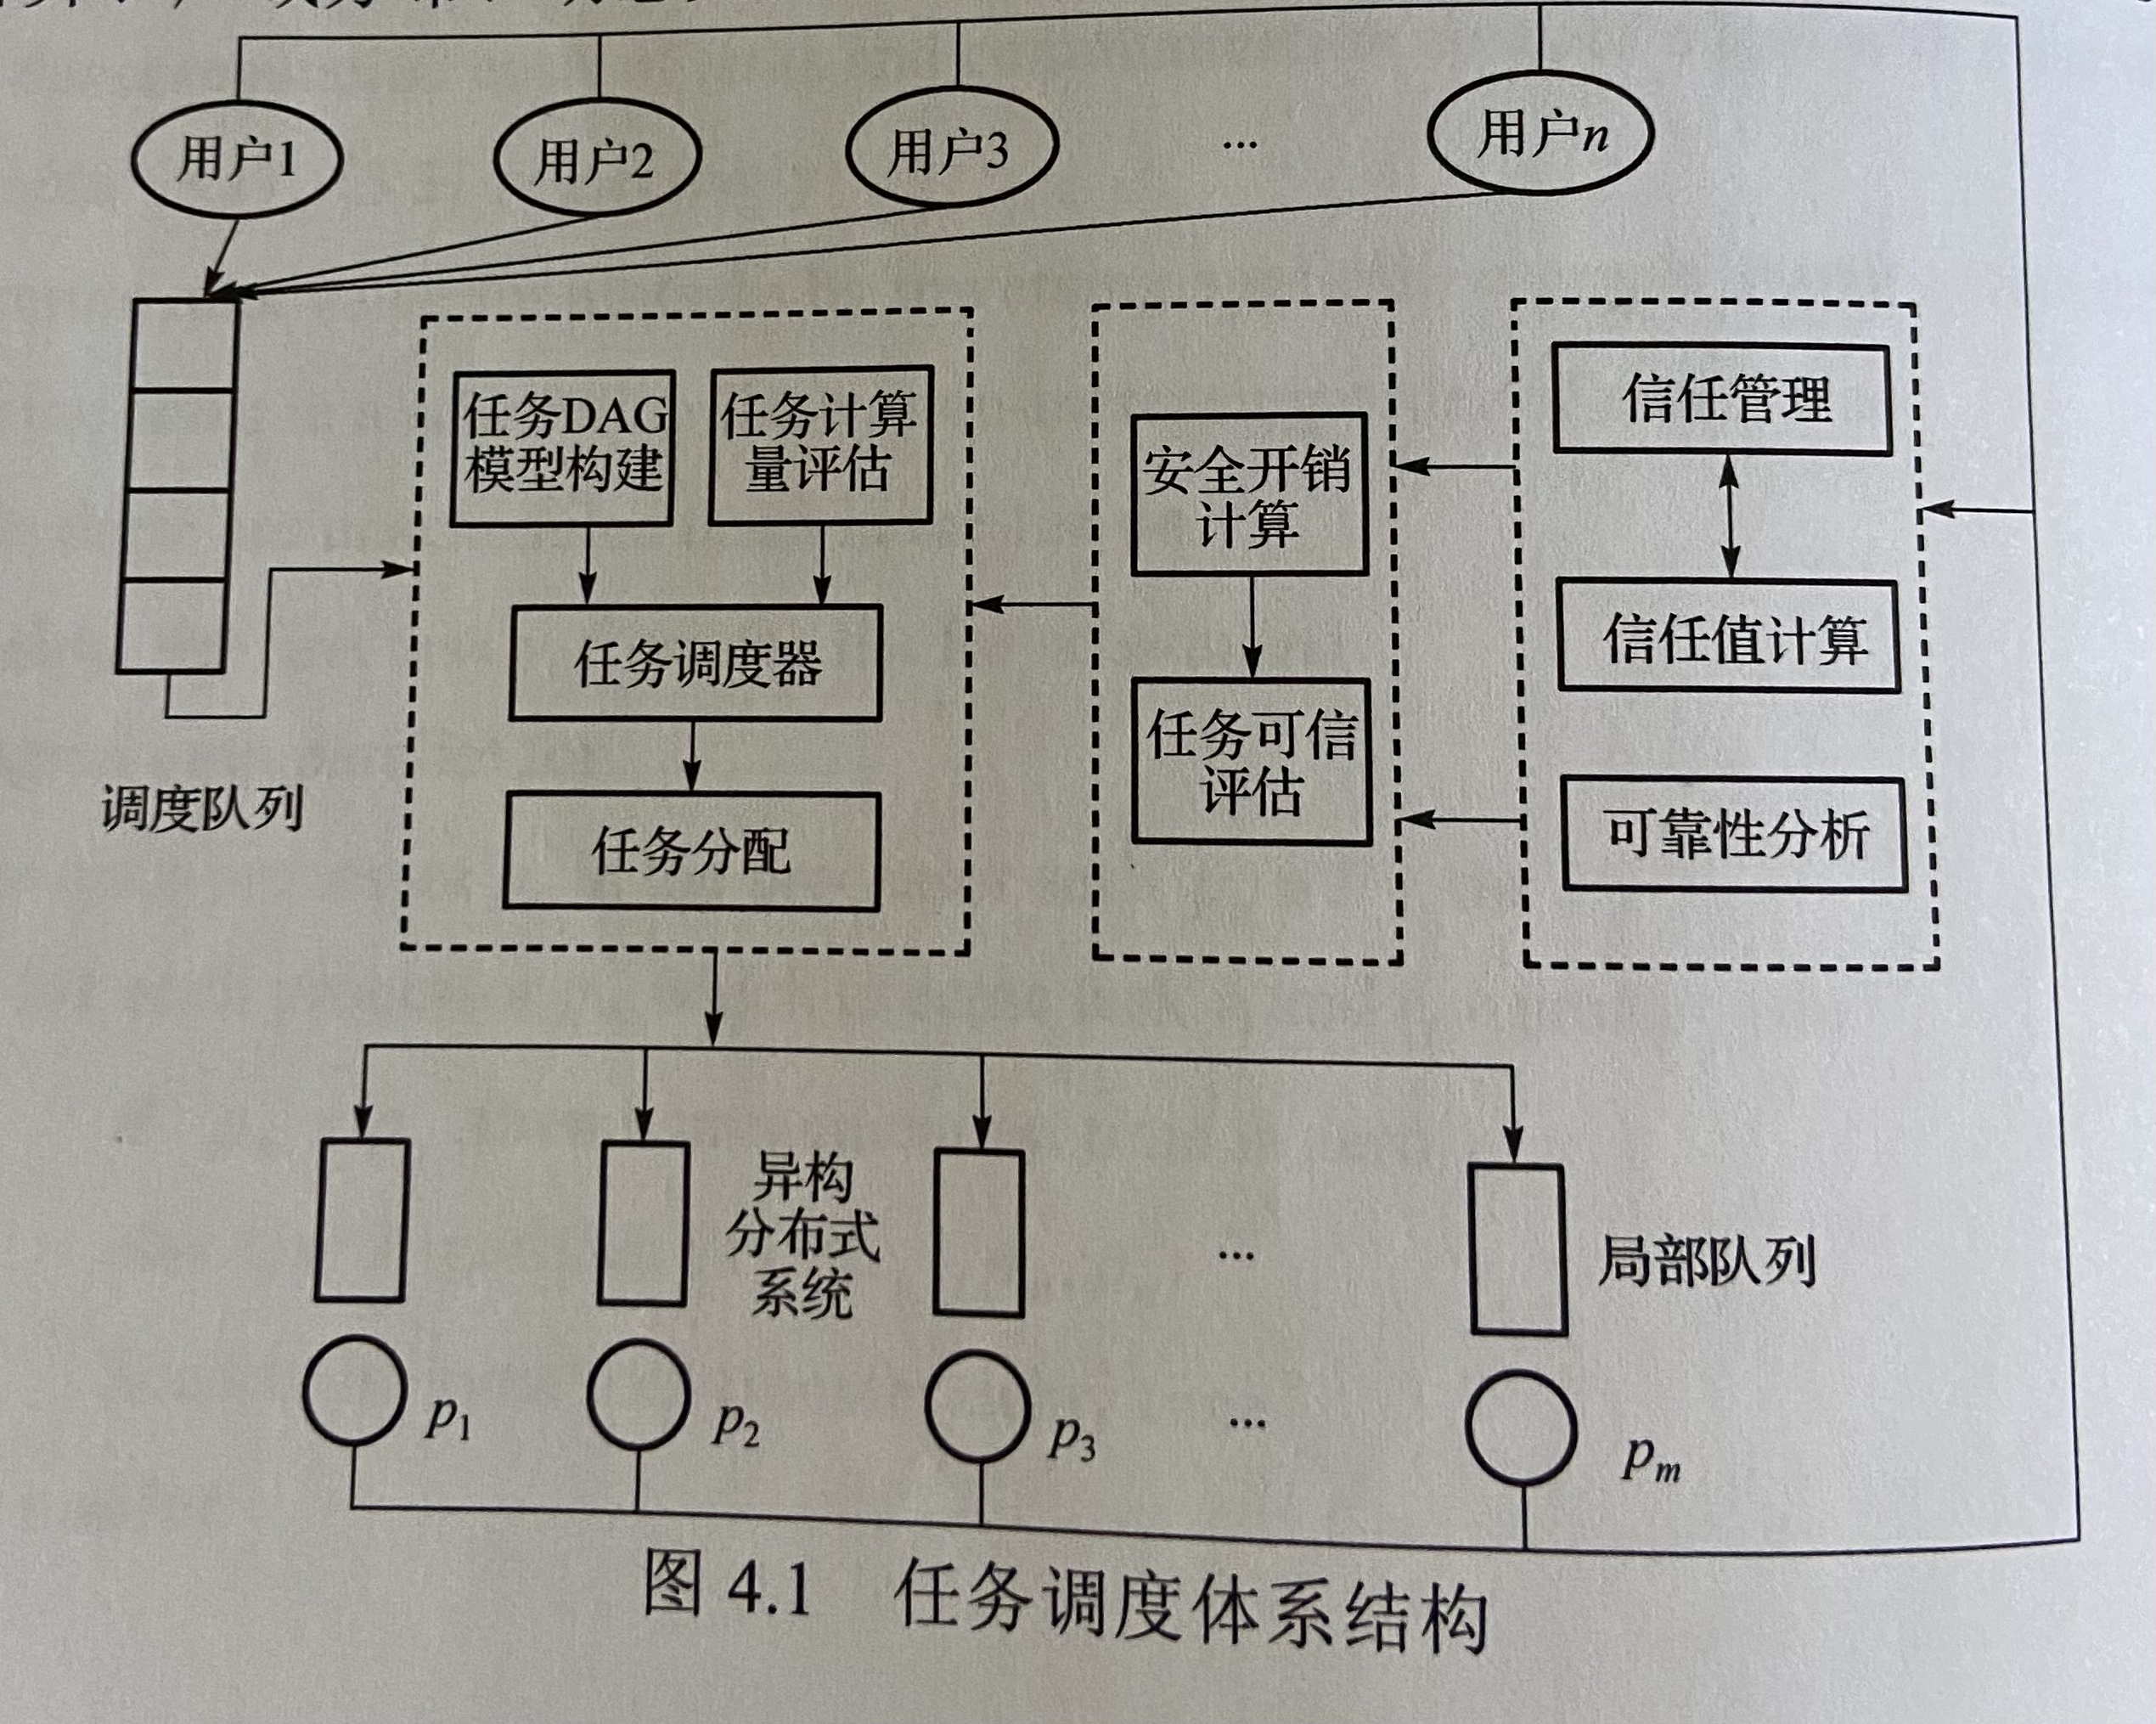
\includegraphics[width=0.8\textwidth]{xiaoyongSchedule.jpg}
\end{figure}
\subsubsection{Sinan: ML-Based and QoS-Aware Resource Management for Cloud Microservices}

\subsection{Super Resolution System}
\subsubsection{Insights:}
\begin{itemize}
    \item Transformer-based Super Resolution Neural Architecture Search and Pruning (AutoFormer: Searching Transformers for Visual Recognition) + ()
\end{itemize}
\subsubsection{Deep Neural Network-based Enhancement for Image and Video Streaming Systems: A Survey and Future Directions}
Visual Delivery System: The primary metrics of interest include essential attributes such as visual quality, frame rate, response time, rebuffering time, accuracy and quality of experience. Visual Quality: by both the bitrate and the amount of computational resources available to execute these models. So the other indexes are the same as the model's. Accuracy, Accuracy is reported as percentage for classification tasks or in the range 0-1 for the Intersection-over-Union (IoU) metric of semantic segmentation tasks;  Response Time Latency, or response time, is the primary performance indicator in latency-sensitive interactive applications, such as virtual reality ; Frame rate; Rebuffering, This phenomenon occurs when the playback buffer is drained due to the slow transmission of video segments. 
\subsubsection{Video Super-Resolution Based on Deep Learning: A Comprehensive Survey}
\subsubsection{SplitSR: An End-to-End Approach to Super-Resolution on Mobile Devices}
\subsubsection{NTIRE 2021 Challenge on Video Super-Resolution}
\subsubsection{Real-Time Single Image and Video Super-Resolution Using an Efficient Sub-Pixel Convolutional Neural Network}
\subsubsection{ImagePairs Building a realistic data set for super-resolution research by using a beam-splitter camera rig}
\subsubsection{https://zhuanlan.zhihu.com/p/263008440 中文blog}
总体:
1)单幅图像分辨率放大 \\
2)从多帧连续图像中重建超分辨率单帧图像;\\
3)视频序列的超分辨率重建。 \\

单幅图像放大主要利用对髙分辨率图像的先验知识和以混叠形式存在的高频信息进行复原。

评价指标:PSNR, 直接对比图像像素差值,它是基于对应像素点间的误差,并未考虑到人眼的视觉特性。因为人眼对空间频率较低的对比差异敏感度较高,对亮度对比差异的敏感度较色度高,人眼对一个区域的感知结果会受到其周围邻近区域的影响,因而经常出现评价结果与人的主观感觉不一致的情况。

SSIM,作为结构相似性理论的实现,结构相似度指数从图像组成的角度将结构信息定义为独立于亮度、对比度的,反映场景中物体结构的属性,并将失真建模为亮度、对比度和结构三个不同因素的组合。用均值作为亮度的估计,标准差作为对比度的估计,协方差作为结构相似程度的度量。

FID, FID(Frechet Inception Distance), IS,即Inception Score,用过Inception, v3模型度量图片分数,可用来算单张图片的分值,越高越好。

1. 频域方法:图像序列被模型化为同一幅场景经整体平移后欠采样的结果,欠采样过程在频域表现为频谱混叠。设F为多帧观测图像傅里叶变换的逐行排列,A:为H标高分辨率图像傅里叶变换的逐行排列,则观测模型可表示为:Y=AX
2. 空域方法
a. 非均匀插值方法
b. 迭代反投影方法
3. 凸集投影方法POCS
4. 随机正则化方法-最大后验概率(MAP)方法

\subsection{ML Huge System}
\subsubsection{TODO LIST:}
1.
\subsubsection{Insights:}
\subsubsection{scaling distributed machine learning with parameter server}
\subsubsection{}

\subsection{Survey of Machine Learning for Computer Architecture and Systems}
\subsubsection{A Survey of Machine Learning for Computer Architecture and Systems}
let ML transform the way that computer architecture and systems are designed. 


\subsection{NAS \& Meta learning in Computer System}
\subsubsection{Insigts:}
\subsubsection{Rethinking and Improving Relative Position Encoding for Vision Transformer}
\subsubsection{Searching the Search Space of Vision Transformer}
\subsubsection{MiniViT: Compressing Vision Transformers with Weight Multiplexing}
\subsubsection{NAS-SE: Designing An Efficient In-Situ One-Shot Neural Architecture Search Engine for Large-Scale Deployment}

\subsection{Graph System}
\subsubsection{Insigts:}
\subsubsection{Krill: A Compiler and Runtime System for Concurrent Graph Processing}
1.Ligra 
2.the time of loading graph nto memory consumes a lot. 

\subsection{Ray}
\subsubsection{Insigts:}
\subsubsection{Ownership: A Distributed Futures System for Fine-Grained Tasks~\cite{wang2021ownership}}
NSDI 2021; The original proposal uses synchronous calls that copy return values back to the caller. It suggest that , we need to pass the results to the master nodes after finish calculating. And in the end, the results will be passed to another nodes. There are too many such processes in the distribution computation. Thus, this process is wasting communication. Several recent systems [4, 34, 37, 45] have extended RPC so that, in addition to distributed communica- tion, the system may also manage data movement and paral- lelism on behalf of the application. Papers:
4. PyTorch - Remote Reference Protocol. \\
5. Ray v1.0. https://github.com/ray-project/ray/ releases/tag/ray-1.0.0.\\
34. Philipp Moritz, Robert Nishihara, Stephanie Wang, Alexey Tumanov, Richard Liaw, Eric Liang, Melih Eli- bol, Zongheng Yang, William Paul, Michael I. Jordan, and Ion Stoica. Ray: A distributed framework for emerg- ing AI applications. In 13th USENIX Symposium on Operating Systems Design and Implementation (OSDI 18), Carlsbad, CA, 2018. USENIX Association.\\
37. Derek G. Murray, Malte Schwarzkopf, Christopher Smowton, Steven Smith, Anil Madhavapeddy, and Steven Hand. CIEL: A universal execution engine for distributed data-flow computing. In Proceedings of the 8th USENIX Conference on Networked Systems Design and Implementation, NSDI’11, pages 113–126, Berke- ley, CA, USA, 2011. USENIX Association.\\
45. Matthew Rocklin. Dask: Parallel computation with blocked algorithms and task scheduling. In Kathryn Huff and James Bergstra, editors, Proceedings of the 14th Python in Science Conference, pages 130 – 136, 2015.\\


\bibliographystyle{unsrt}
\bibliography{reference}
\end{document}